\documentclass[a4pper,11pt,onecolumn]{article}
\setlength\parindent{2em}
\usepackage{graphicx}
\usepackage{authblk}
\usepackage{pythonhighlight}


\usepackage{hyperref}
\hypersetup{
	colorlinks=true,
	linkcolor=blue,
	filecolor=blue,      
	urlcolor=blue,
	citecolor=cyan,
}

\title{Group Practical 1 }
\author[*]{Shiyu Yi,2016141231175\\Chuang Du,2016141462277\\Jiali Shang,2016141462137}

\renewcommand\Authands{ and }

\begin{document}

\maketitle

%section
\section{Problem overview}
1. Using iris data to assess the classification performance by tuning the KNN
classifiers:

• Splitting the data using different percentage

• Change cross validation folds

• Changing the value of K

• Normalise the data

1) Summarise the above classification performances of the above settings
using tables/figures 

2) Discuss the results.
 
\section{Problem one}

The data of the table 1 is from weka, we can see 

1. When the percentage of traning is 0.4, the evaluate score is the highest, which means when we use half of the data to train and the other half to test, the model performs best.

2. When the percentage of traning is 0.1, the evaluate score is the lowest.

3. When the trainning part goes from 0.9 to 0.4, the evaluate score goes up.

4. when the trainning part goes from 0.4 to 0.1, the evaluate score goes down.
We could find when the percentage is 0.4, the model has highest Correctly Classified Instances,TP rate,Precision,Recall,F-Measure,MCC,ROC Area, PRC Area and the lowest FP rate.


This data is from the software weka:
 
\begin{table}[h]  %table 里面也可以嵌套tabular,只有tabular是不能加标题的
	\centering  %表格居中
	\caption{Splitting the data using different percentage(weka)}  %表格标题
	\begin{tabular}{cccc}  %右对齐
		\hline
		\hline
		& Training proportion & Test Proportion & Evaluate Score \\ [0.5ex] 
		\hline
		& 0.9 & 0.1 & 0.933333   \\
		& 0.8 & 0.2 & 0.966667  \\
		& 0.7 & 0.3 & 0.955556  \\
		& 0.6 & 0.4 & 0.950000    \\
		& 0.5 & 0.5 & 0.96000 \\
		& 0.4 & 0.6 & 0.966667\\
		& 0.3 & 0.7 & 0.942857 \\
		& 0.2 & 0.8 & 0.958333  \\
		& 0.1 & 0.9 & 0.903704  \\
		\hline
		\hline
	\end{tabular}
\end{table}

\begin{table}[h] 
	\centering  
	\caption{The Detailed Accuracy(From weka) }  %表格标题
	\begin{tabular}{ccccccccc}  
		\hline
		\hline
		Percentage & TP Rate & FP Rate & Precision & Recall & F-Measure & MCC   & ROC   & PRC   \\ [0.5ex] 
		\hline
		0.1        & 0.904   & 0.048   & 0.904     & 0.904  & 0.904     & 0.856 & 0.928 & 0.854 \\
		0.2        & 0.958   & 0.022   & 0.960     & 0.958  & 0.958     & 0.937 & 0.968 & 0.934 \\
		0.3        & 0.943   & 0.025   & 0.952     & 0.943  & 0.943     & 0.919 & 0.960 & 0.916 \\
		0.4        & 0.967   & 0.014   & 0.970     & 0.967  & 0.967     & 0.952 & 0.977 & 0.949 \\
		0.5        & 0.960   & 0.021   & 0.964     & 0.960  & 0.960     & 0.941 & 0.970 & 0.939 \\
		0.6        & 0.950   & 0.027   & 0.956     & 0.950  & 0.950     & 0.926 & 0.962 & 0.925 \\
		0.7        & 0.956   & 0.025   & 0.960     & 0.956  & 0.955     & 0.935 & 0.966 & 0.931 \\
		0.8        & 0.967   & 0.017   & 0.970     & 0.967  & 0.966     & 0.953 & 0.976 & 0.947 \\
		0.9        & 0.933   & 0.033   & 0.944     & 0.933  & 0.933     & 0.906 & 0.953 & 0.902\\
		\hline
		\hline
	\end{tabular}
\end{table}

To compare we use the sklean to train the data:\\

The code:\url{https://github.com/chanchann/Bio_Machine_Learning}\\

\begin{table}[h]  %table 里面也可以嵌套tabular,只有tabular是不能加标题的
	\centering  %表格居中
	\caption{Splitting the data using different percentage(sklearn)}  %表格标题
	\begin{tabular}{cccc}  %右对齐
		\hline
		\hline
		& Training proportion & Test Proportion & Evaluate Score \\ [0.5ex] 
		\hline
		 & 0.9 & 0.1 & 0.9333333333333333  \\
		 & 0.8 & 0.2 & 0.9333333333333333 \\
		 & 0.7 & 0.3 & 0.9555555555555556 \\
		 & 0.6 & 0.4 & 0.9666666666666667 \\
		 & 0.5 & 0.5 & 0.9733333333333334 \\
		 & 0.4 & 0.6 & 0.9666666666666667\\
		 & 0.3 & 0.7 & 0.9333333333333333 \\
		 & 0.2 & 0.8 & 0.9166666666666666 \\
		 & 0.1 & 0.9 & 0.837037037037037 \\
		\hline
		\hline
	\end{tabular}
\end{table}

By the table3 which is the result of codes, we can see\\

1.when the percentage of traning is 0.5, the evaluate score is the highest, which means when we use half of the data to train and the other half to test, the model performs best.

2.when the percentage of traning is 0.1, the evaluate score is the lowest.

3.when the trainning part goes from 0.9 to 0.5, the evaluate score goes up.

4.when the trainning part goes from 0.5 to 0.1, the evaluate score goes down.

The difference may caused by many aspects such as parameters,evaluate methods and so on.

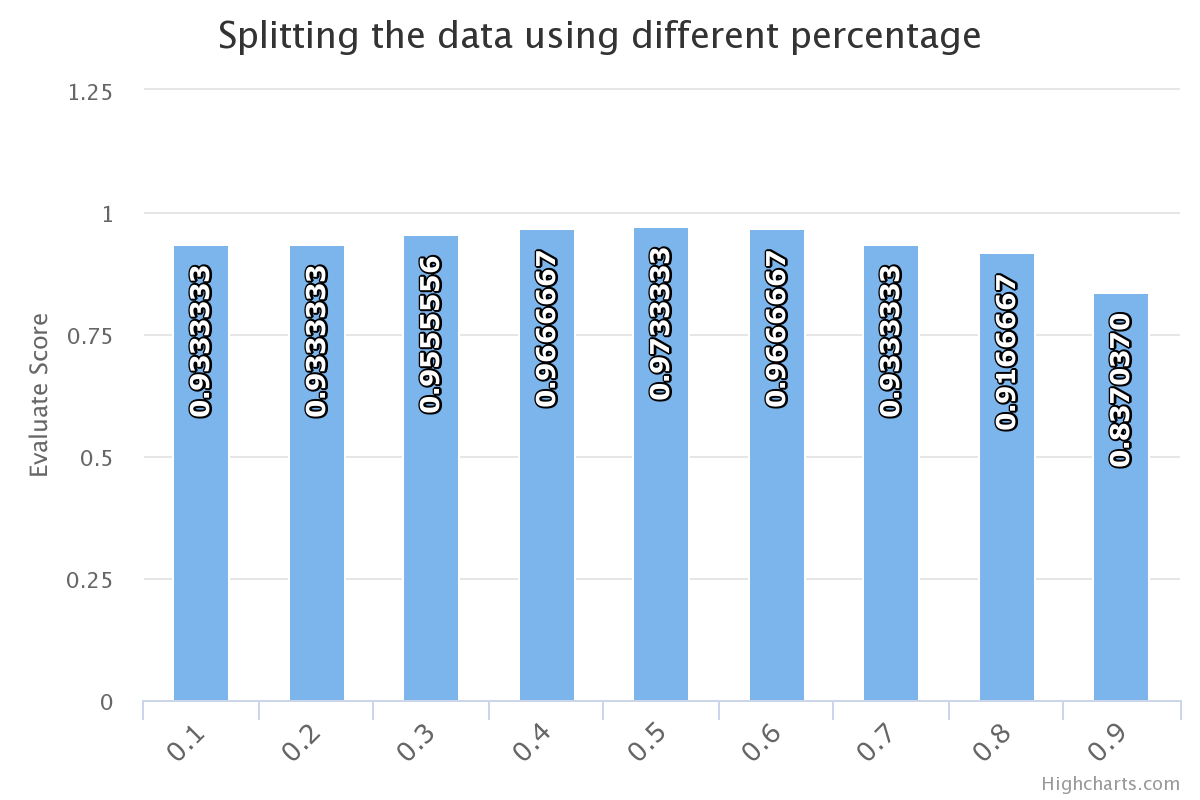
\includegraphics[width=\linewidth]{split.png}


\section{Problem two}

\begin{table}[h] 
	\centering  
	\caption{The cross validation folds Detailed Accuracy }  %表格标题
	\begin{tabular}{ccccccccc}  
		\hline
		\hline
		Fold & TP Rate & FP Rate & Precision & Recall & F-Measure & MCC   & ROC   & PRC   \\ [0.5ex] 
		\hline
	2    & 0.940   & 0.030   & 0.941     & 0.940  & 0.940     & 0.911 & 0.956 & 0.907 \\
	3    & 0.947   & 0.027   & 0.947     & 0.947  & 0.947     & 0.920 & 0.961 & 0.917 \\
	4    & 0.960   & 0.020   & 0.960     & 0.960  & 0.960     & 0.940 & 0.985 & 0.962 \\
	5    & 0.940   & 0.030   & 0.941     & 0.940  & 0.940     & 0.911 & 0.957 & 0.907 \\
	6    & 0.953   & 0.023   & 0.953     & 0.953  & 0.953     & 0.930 & 0.966 & 0.927 \\
	7    & 0.947   & 0.027   & 0.947     & 0.947  & 0.947     & 0.920 & 0.963 & 0.924 \\
	8    & 0.960   & 0.020   & 0.960     & 0.960  & 0.960     & 0.940 & 0.978 & 0.949 \\
	9    & 0.953   & 0.023   & 0.953     & 0.953  & 0.953     & 0.930 & 0.972 & 0.937\\
		\hline
		\hline
	\end{tabular}
\end{table}


By the data from weka we can see that

1. when the fold is set as 4, it has the the model hashighest Correctly Classified Instances,TP rate,Precision,Recall,F-Measure,MCC,ROC Area, PRC Area and the lowest FP rate.
If we take ROC area as the standard for judging accuracy,we would find

2. when the fold goes from 2 to 4, the ROC area is rising overall.

3. when the fold goes from 4 to 5, the ROC area is reduced .

4. when the fold goes from 5 to 9, the ROC area is rising again but the peak has never reached as high as when fold is 4.


\begin{table}[h]  
	\centering  
	\caption{cross validation folds(From Sklearn)}  
	\begin{tabular}{cccc} 
		\hline
		\hline
		& cv's folder & Accuracy  \\ [0.5ex] 
		\hline
		& 2 & 0.94(+/-0.04)   \\
		& 3 & 0.99(+/-0.02)  \\
		& 4 & 0.97(+/-0.04)  \\
		& 5 & 0.97(+/-0.05)  \\
		& 6 & 0.97(+/-0.07) \\
		& 7 & 0.97(+/-0.07) \\
		& 8 & 0.97(+/-0.08) \\

		\hline
		\hline
	\end{tabular}
\end{table}



By the table5 we can see that\\

1. when the fold is  set as 3, the model has the highest accuracy

2. when the fold goes up from 3 to 8, the accuracy goes down

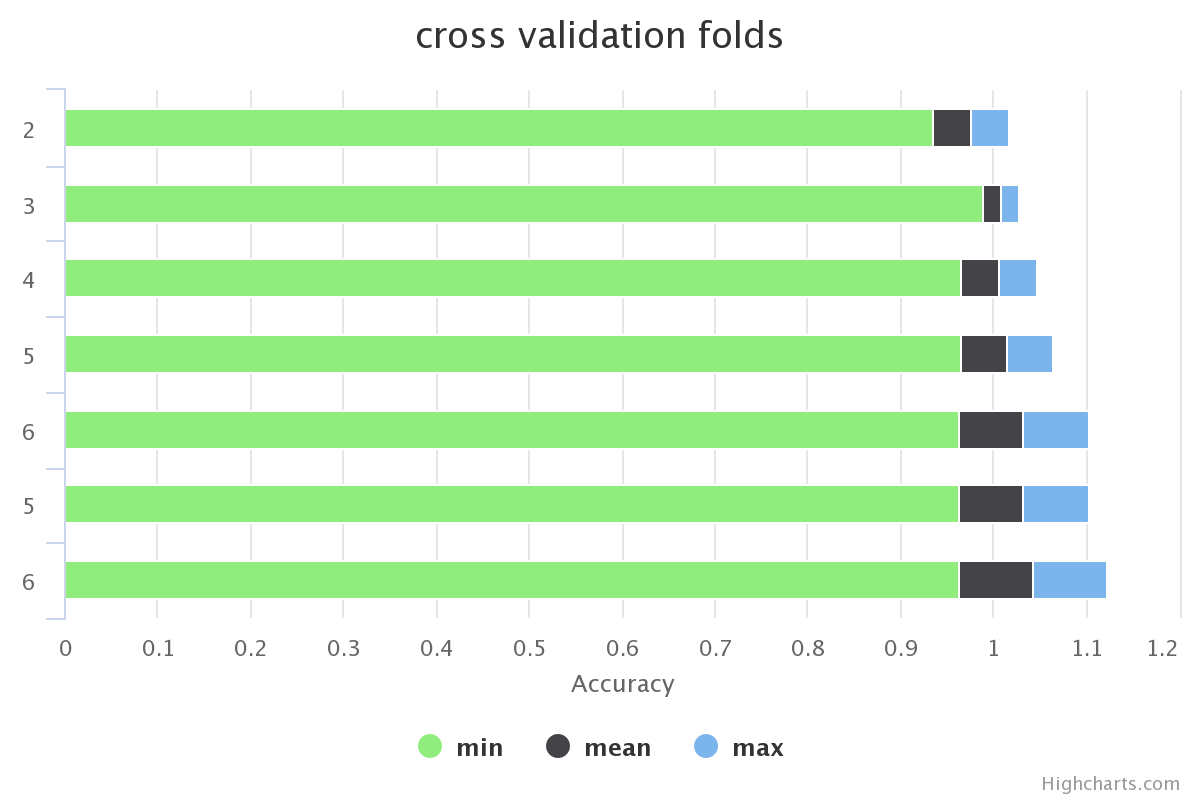
\includegraphics[width=\linewidth]{cross.png}

\section{Problem three}

\begin{table}[h] 
	\centering  
	\caption{The different K's Detailed Accuracy }  %表格标题
	\begin{tabular}{ccccccccc}  
		\hline
		\hline
		K & TP Rate & FP Rate & Precision & Recall & F-Measure & MCC   & ROC   & PRC   \\ [0.5ex] 
		\hline
		1 & 0.960   & 0.020   & 0.960     & 0.960  & 0.960     & 0.940 & 0.985 & 0.962 \\
		2 & 0.960   & 0.020   & 0.960     & 0.960  & 0.960     & 0.940 & 0.986 & 0.966 \\
		3 & 0.953   & 0.023   & 0.953     & 0.953  & 0.953     & 0.930 & 0.987 & 0.969 \\
		4 & 0.960   & 0.020   & 0.960     & 0.960  & 0.960     & 0.940 & 0.985 & 0.972 \\
		5 & 0.960   & 0.020   & 0.960     & 0.960  & 0.960     & 0.940 & 0.991 & 0.979 \\
		6 & 0.960   & 0.020   & 0.960     & 0.960  & 0.960     & 0.940 & 0.996 & 0.992 \\
		7 & 0.953   & 0.023   & 0.953     & 0.953  & 0.953     & 0.930 & 0.997 & 0.994 \\
		8 & 0.960   & 0.020   & 0.960     & 0.960  & 0.960     & 0.940 & 0.998 & 0.995 \\
		9 & 0.960   & 0.020   & 0.960     & 0.960  & 0.960     & 0.940 & 0.997 & 0.993\\
		\hline
		\hline
	\end{tabular}
\end{table}

We choose ROC area as the criterion for judging the accuracy of the model.
By the table we can see that,

1. when K =8, the model has the highest ROC Area.

2. when K goes from 1 to 8, and the ROC area is rising overall.

\section{Problem Four}

We use the different nomalization method to dicovery the effect:

\begin{table}[h]  
	\centering  
	\caption{Normalise the data(code)}  
	\begin{tabular}{cccc} 
		\hline
		\hline
		& Method & Accuracy  \\ [0.5ex] 
		\hline
		& Min-Max scaling & 0.97(+/-0.05)   \\
		& Standardization & 0.97(+/-0.02)  \\
		& Normalizer & 0.97(+/-0.04)  \\
		\hline
		\hline
	\end{tabular}
\end{table}

By the table7 we can see that, the Standardization has the minimum fluctuation interval.

\section{Classification}

We can plot the graph to see the Data distribution
\\
\\
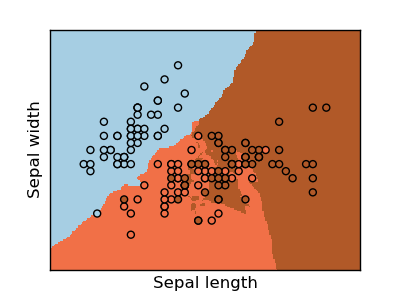
\includegraphics[width=\linewidth]{plot_knn_iris_1.png}


\section{Discussion}

In our case, we chose the ROC area as a standard for judging models.
ROC area is a curve, and the area covered under this curve on the coordinate axis is approximately close to 1, indicating that the prediction of the model is better.

We can find that if we set 0.4 as our percentage, 4 as our fold and 8 for the K value, the ROC area is more close to 1, so this model will have the highest accuracy.

Due to the random selection of seeds, the data obtained from each run would differ slightly, but the overall accuracy was not affected.

\section{Code}

split.py\\
To implement Splitting the data using different percentage

\begin{python}
	import numpy as np
	import pandas as pd
	from sklearn import datasets
	from sklearn.neighbors import KNeighborsClassifier
	
	iris=datasets.load_iris()
	iris_x=iris.data
	iris_y=iris.target
	
	# Split iris data in train and test data
	# A random permutation, to split the data randomly
	
	np.random.seed(0)
	indices=np.random.permutation(len(iris_x))
	for i in np.arange(0.1,1,0.1):
	test_size=-1*i*len(indices)
	test_size=int(test_size)
	iris_x_train=iris_x[indices[:test_size]]
	iris_y_train=iris_y[indices[:test_size]]
	iris_x_test=iris_x[indices[test_size:]]
	iris_y_test=iris_y[indices[test_size:]]
	#Create a nearest-neighbor classifier
	knn=KNeighborsClassifier()
	knn.fit(iris_x_train,iris_y_train)
	#iris_x_predict=knn.predict(iris_x_test)
	#print(iris_x_predict)
	#print(iris_y_test)
	score=knn.score(iris_x_test,iris_y_test)
	#print(score)
	print('test proprotion: {0},\nevaluate score:{1}'.format(i,score))
	print('-------------------------------------------------')
\end{python}

crossVal.py\\

To use cross validation folds.

\begin{python}
	import numpy as np
	import pandas as pd
	from sklearn import datasets
	from sklearn.neighbors import KNeighborsClassifier
	from sklearn.model_selection import train_test_split
	from sklearn.model_selection import cross_val_score
	
	#Create the KNNClassifer
	knn=KNeighborsClassifier()
	# knn.fit(x_train,y_train)
	for i in range(2,9):
	scores=cross_val_score(knn,iris.data,iris.target,cv=i)
	print(scores)
	print("Accuracy:%0.2f(+/-%0.2f)"%(scores.mean(),scores.std()*2))
	print("----------------------------------------------")
\end{python}


normalize.py\\

To normalize the data to train.

\begin{python}
	import numpy as np
	import pandas as pd
	from sklearn import datasets
	from sklearn.neighbors import KNeighborsClassifier
	from sklearn.model_selection import train_test_split
	from sklearn.model_selection import cross_val_score
	from sklearn.preprocessing import MinMaxScaler
	from sklearn.preprocessing import StandardScaler
	from sklearn.preprocessing import Normalizer
	
	iris=datasets.load_iris()
	#Min-Max scaling
	#MinMaxScaler().fit_transform(iris.data)
	
	#Standardization
	# StandardScaler().fit_transform(iris.data)
	
	# Normalizer
	Normalizer().fit_transform(iris.data)
	
	# Here we split the data 0.6:0.4
	x_train,x_test,y_train,y_test=train_test_split(
	iris.data,iris.target,test_size=0.4,random_state=0)
	
	#Create the KNNClassifer
	knn=KNeighborsClassifier()
	scores=cross_val_score(knn,iris.data,iris.target,cv=5)
	print("Accuracy:%0.2f(+/-%0.2f)"%(scores.mean(),scores.std()*2))
\end{python}

plot.py\\

To plot the classification.

\begin{python}
	import numpy as np
	import pylab as pl
	from sklearn import neighbors, datasets
	
	# import some data to play with
	iris = datasets.load_iris()
	X = iris.data[:, :2] # we only take the first two features. 
	Y = iris.target
	
	
	h = .02 # step size in the mesh
	
	knn=neighbors.KNeighborsClassifier()
	
	# we create an instance of Neighbours Classifier and fit the data.
	knn.fit(X, Y)
	
	# Plot the decision boundary. For that, we will asign a color to each
	# point in the mesh [x_min, m_max]x[y_min, y_max].
	x_min, x_max = X[:,0].min() - .5, X[:,0].max() + .5
	y_min, y_max = X[:,1].min() - .5, X[:,1].max() + .5
	xx, yy = np.meshgrid(np.arange(x_min, x_max, h), np.arange(y_min, y_max, h))
	Z = knn.predict(np.c_[xx.ravel(), yy.ravel()])
	
	# Put the result into a color plot
	Z = Z.reshape(xx.shape)
	pl.figure(1, figsize=(4, 3))
	pl.set_cmap(pl.cm.Paired)
	pl.pcolormesh(xx, yy, Z)
	
	# Plot also the training points
	pl.scatter(X[:,0], X[:,1],c=Y )
	pl.xlabel('Sepal length')
	pl.ylabel('Sepal width')
	
	pl.xlim(xx.min(), xx.max())
	pl.ylim(yy.min(), yy.max())
	pl.xticks(())
	pl.yticks(())
	
	pl.show()	
\end{python}


\end{document}